% This template has been tested with LLNCS DOCUMENT CLASS -- version 2.20 (10-Mar-2018)

% !TeX spellcheck = en-US
% !TeX encoding = utf8
% !TeX program = pdflatex
% !TeX TXS-program:compile = txs:///pdflatex/[--shell-escape]
% !BIB program = bibtex
% -*- coding:utf-8 mod:LaTeX -*-

% German documents: pass ngerman as class option
% \documentclass[ngerman,runningheads,a4paper]{llncs}[2018/03/10]
% English documents: pass english as class option
\documentclass[ngerman,runningheads,a4paper]{llncs}[2018/03/10]

\usepackage{improved-lncs}

\begin{document}

\title{Subsurface scattering: Kombination von Theorie und Implementierungstechniken am Beispiel des realistischen Renderns von Haut}
%If Title is too long, use \titlerunning
\titlerunning{Realitische Echtzeitdarstellung von Haut}

%Single insitute
\author{Dennis Grabowski, B.Sc.}
%If there are too many authors, use \authorrunning
\authorrunning{D. Grabowski}

\institute{Hochschule Hannover, Ricklinger Stadtweg 120, 30459 Hannover, Germany\\
\email{dennis.grabowski@stud.hs-hannover.de}\\
\url{https://f4.hs-hannover.de/}}

\maketitle

\begin{abstract}
  Unter dem typischen Phong-Modell ist es schwer, verschiedenste Materialien wie Marmor, Wachs, Blätter oder Haut realistisch dar\-zu\-stellen.
  Zugrunde liegt, dass das Phong-Modell nur ein empirisches Model ist und keineswegs ein physikalisch haargenaues Modell darstellt, wodurch verschiedenste physikalische Effekte schlichtweg nicht nachstellbar sind.
  Diese Ausarbeitung wird ausleuchten, welche Schwierigkeiten sich ergeben, Haut realistisch darzustellen und welche Konzepte helfen, diesen Realismus wiedergeben zu können.
  Haut als Medium bietet sich besonders an, um an diese Konzepte heranzugehen, da jedem Leser hoffentlich eine realistische Präsentation dieser bekannt ist.
  Hierfür wird zunächst aufgezeigt, wie Licht mit Haut interagiert, um die physikalischen Grundlagen der sogenannten Volumenstreuung (engl. subsurface scattering) kennenzulernen.
  Anschliessend werden bestehende Techniken angeschnitten, die dieses physikalische Phänomen auf verschiedenste Weisen implementieren.
  Durchleuchtet wird die sogenannte \enquote{Texture-space Diffusion}, welche bereits fuer den Film \enquote{The Matrix} verwendet wurde und von NVIDIA's d'Eon und Luebke fuer ein Echtzeit-Rendering-System adaptiert wurde.
  Diese Technik verwendet die bidirektionale Reflexionsverteilungsfunktion von Kelemen und Szirmay-Kalos, um eine realistische Oberflächenreflexion zu simulieren, sowie Diffusionsprofile und Translucent Shadow Maps, um die Auswirkungen des Subsurface Scattering auf dem Hautmaterial nachzuahmen.
  Nachfolgend werden Bilder verschiedenster Implementationen sowie aktuellere Ergebnisse von \enquote{Offline-Renderern} miteinander vergliechen, um die Wirkung dieser Konzepte besser einschätzen zu können.
\end{abstract}

\begin{keywords}
  Computergrafik, Physikalisch-basiertes Rendering, Bidirektionale Reflexionsverteilungsfunktions (BRDFs), Subsurface scattering (deutsch Unterirdische Streuung/Volumenstreuung), Diffusionsprofile, Translucent shadow maps
\end{keywords}

\section{Einleitung}
\label{sec:intro}

describe
refraction,
refractive index as a complex number
homogeneous (glass, crystals, water, oil, wine) medium
absorbed light travels through them, but do not change direction, only intensity
homogeneous materials do not succumb to subsurface scattering
heterogenous medium (wood, stone, snow, earth, skin, opaque plastic) is the interesting part for us
contains numerous discontinuities - air bubbles, foreign particles, density variations, structural changes


\section{Subsurface scattering}
\label{sec:subsurface}

 scattering occurs when suddenly change of refractive index happens
 scattering does not change "amount" of light, only directions
 scattering distribution depends on type of material and is non-uniform

 now - what happens to the refracted light
   depends on the material
     metals fully absorb the refracted light, causing it to get hotter
     non-metals (aks dielectrics/insulators) play by the same rules as learned until now - absorption, scattering happens
       absorption obeys exponential decay law with respect to total travel distance through material (real-time rendering 9.4)
         spectrally variant, i.e. different RGB values
       scattering is similarly, probability of light not being scattered obeys an exponential decay law with distance.
         normally no dependence on wavelength, but sometimes the discontinuities decide the spectral variants - i.e. blue light scatters more often than red light, which makes the sky blue?
   some refracted light is scattering such that it is re-emitted out of the same surface - but often from a different spot than the original entrance.
   some of the refracted light is scattering in the material and will never be re-emitted as it scatters until enough light will be absorbed inside the material

\subsection{Konzeptionelle Adapation von Volumenstreuung in der Computergrafik}

 applying these to computer graphics, we find a difference in where the re-emitted light will emerge from the material based on the pixel size (use figure 17 from physics shading)
       if light exits in the same pixel, we can disregard the distance between their re-emitted exit and the original entrance - choose original entrance as exit. now, a local shading technique could be used.
         This assumption is needed for a BRDF, also called local subsurface scattering
         this interesting fact btw allows us to use diffuse shading techniques for skin of a distant character,
       the other case is that the exit of the re-emitted light is inside another pixel, i.e. the distance to the original point of entry is larger than one pixel, which means that the shading of each point is depending on all points in his neighborhood.
         for this case, the subsurface scattering techniques have been developed as now a BRDF cannot model the different points of exit for each scattered light ray
         here, a global illumination model is needed
     math behind this only concerns radiance, i.e. magnitude of light along a single ray
       is a spectral quantity: amount varies as a function of wave length
       $L_i$ incoming to surface
       $L_o$ outgoing from surface
       $v$ denotes a unit-length vector pointing along the outgoing direction
       $l$ denotes a unit-length vector pointing opposite to the incoming direction
         it is more convenient to have all vectors point away from the surface
       $n$ denotes surface normal vector
   subsurface scattering
     definitions
       scattering albedo p is ratio between energy of light that escapes a surface compared to energy of light entering into the material
         value is between 0 (all light absorbed) and 1 (no light absorbed)
         fresh snow or foam on liquid is good example of high scattering albedo - little absorption, immense scattering
         good to know/consider is that albedo can have a different spectral distribution and thus color - think of plastic: reflecting specularly light is white, while reflecting diffusely will be colored by the pigment particles of the plastic (i.e. blue)
         https://de.wikipedia.org/wiki/Albedo
     local/global
       local subsurface scattering is often a Lambert BRDF:
         $f_diff(l, v) = c_diff / pi$
         or based on fresnel's effect, specular reflectance increases at glancing angles, diffuse reflectance decreases: $f_diff(l, v) = (1 - R_F(Pho_i))  p_albedo/pi$
         remember - here we consider point of exit to be the same as point of entry, i.e. each pixel can be calculcated individually
       global subsurface scattering:
         here, we consider, that each vertex/pixel can influence the shading in neighbor pixels
     difference in bounce consideration
       single-bounce subsurface scattering
         scatters once before leaving the material
       multiple-bounce subsurface scattering
         scatters twice, three times or more often
       for most materials, single scattering is relatively weak part of total scattering effect, multipe scattering predominate - skin is such an example
       most subsurface scattering rendering techniques therefore focus on simulating multiple scattering

\section{Bekanntesten Techniken zum Rendern von realistischer Haut}
\label{sec:application}

\subsection{A Spectral BSSRDF for Shading Human Skin}
\label{sub:spectral-bssrdf}

\citet{spectral-bssrdf-human-skin}

 BSSRDF - bidirectional surface scattering distrubition function, by Jensen et al. 2001
         light distribution tends to be isotropic in a highly scattering media - i.e. once light is in the surface, it's randomly likely to end up coming out any direction rather being mostly aligned to the incoming light direction or any other similar possible dependency term
           this makes scattering sort of a blurring function
             comes from stam, 1995 - multiple scattering as a diffusion profile
           based on two parts:
             one method for exact computation of single-scattering contribution
             dipole method that approximates the multiple-scattering contribution by evaluating two virtual point light sources, one below and one above the surface

\subsection{Pre-Integrated Deferred Subsurface Scattering}
\label{sub:pre-integrated}

\citet{pre-integrated-subsurface}

\subsection{Screen-space perceptual rendering of human skin}
\label{sub:screen-space}

\citet{screen-space-subsurface}

\section{Texture-Space Diffusion}
\label{sec:texture-space}

 Texture-Space Diffusion
 based on an technique called Normal blurring
   an idea by Ma et al based on measured data that showed reflected lights from scattered objects specular reflecntance is based on geometric surface normals, diffuse reflectance behave as if it uses blurred surface normals
 a technique popularized by Borshukov and Lewis for the film Matrix
 formalizes the idea of multiple scattering as a blurring process of a texture
 surface irradiance aka diffuse lighting is rendered into a texture
   done by using texture coordinates as positions for rasterization.
   this texture is then blurred and used for diffuse shading when rendering
   shape/size of filter for blurring depends on material and wavelength
     for skin, a wider filter is used on R channel than on G or B channel causing the reddening near shadow edges
     most often, correct filter has narrow spike in the center, wide shallow base
 this technique is very expensive, requiring large number of blurring passes - scaling back is possible for performance, but comes at a cost of realism

\citet{efficient-human-skin-rendering}
It's called "texture-space" because all of the scattering/diffusion simulation happens in 2D using the UV parameterization

FaceBreaker / Fight Night \url{https://images9.gry-online.pl/galeria/galeria_duze3/2145344968.jpg} used Texture-Space Diffusion \url{https://twitter.com/vicki_ferg/status/1181069047053635584?s=20}

\subsection{Skin surface reflected light}
\label{sub:skin-surface-reflect}

\subsection{Skin subsurface reflected light}
\label{sub:skin-subsurface-reflect}

\subsection{Skin model used}
\label{sub:skin-model}

\subsection{Diffusion profiles}
\label{sub:diffusion-profiles}

\subsection{Translucent shadow maps}
\label{sub:translucent-shadow-maps}

\citet{translucent-shadow-maps}

\section{Conclusion and Outlook}
\label{sec:outlook}

 Volumetric path tracer, used by Pixar/Disney or Framestore (VFX studio behind GotG2 / Alien: Covenant)
 too expensive for games/anything interactive

\begin{figure}
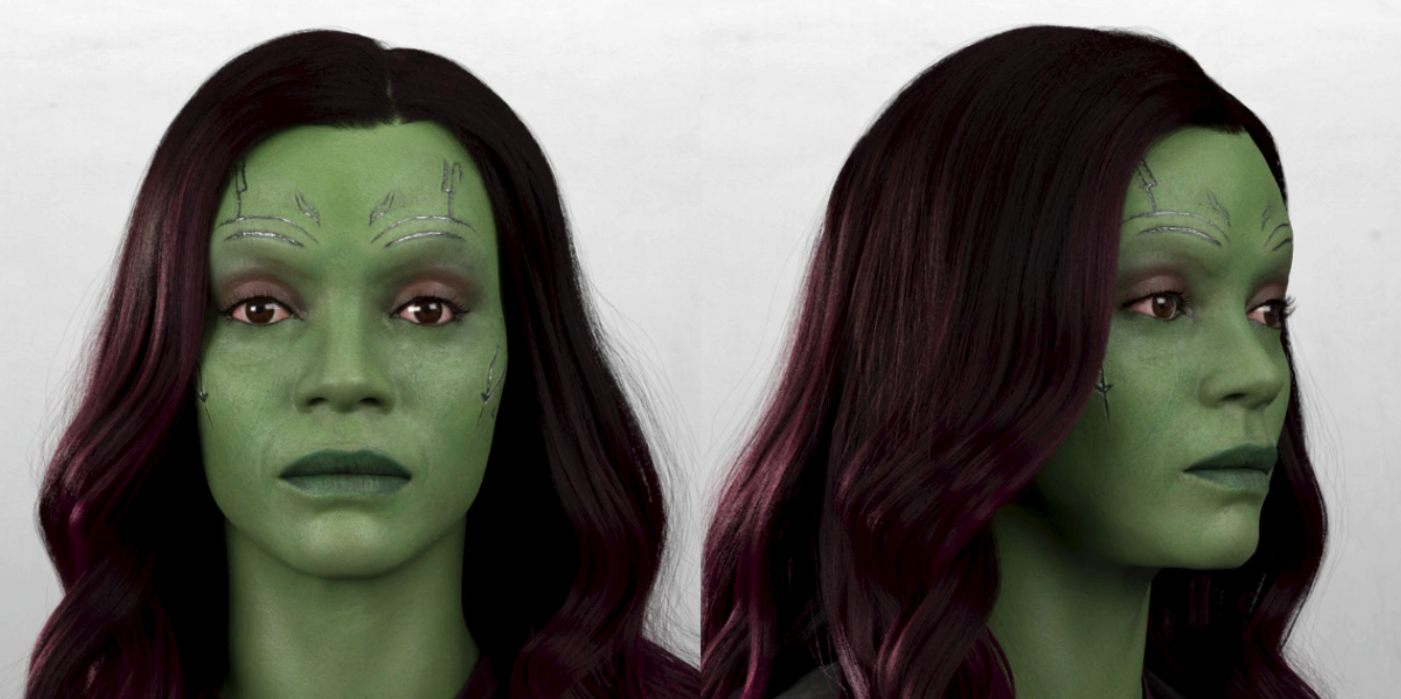
\includegraphics[scale=0.275,keepaspectratio]{./images/framestore-digital-gamora.jpg}
\caption{Volumetric path tracer - technique used by Framestore \protect\footnotemark}
\footnotetext{Quelle: \url{https://blog.selfshadow.com/publications/s2017-shading-course/walster/s2017_pbs_volumetric_notes.pdf}}
\end{figure}

\begin{figure}
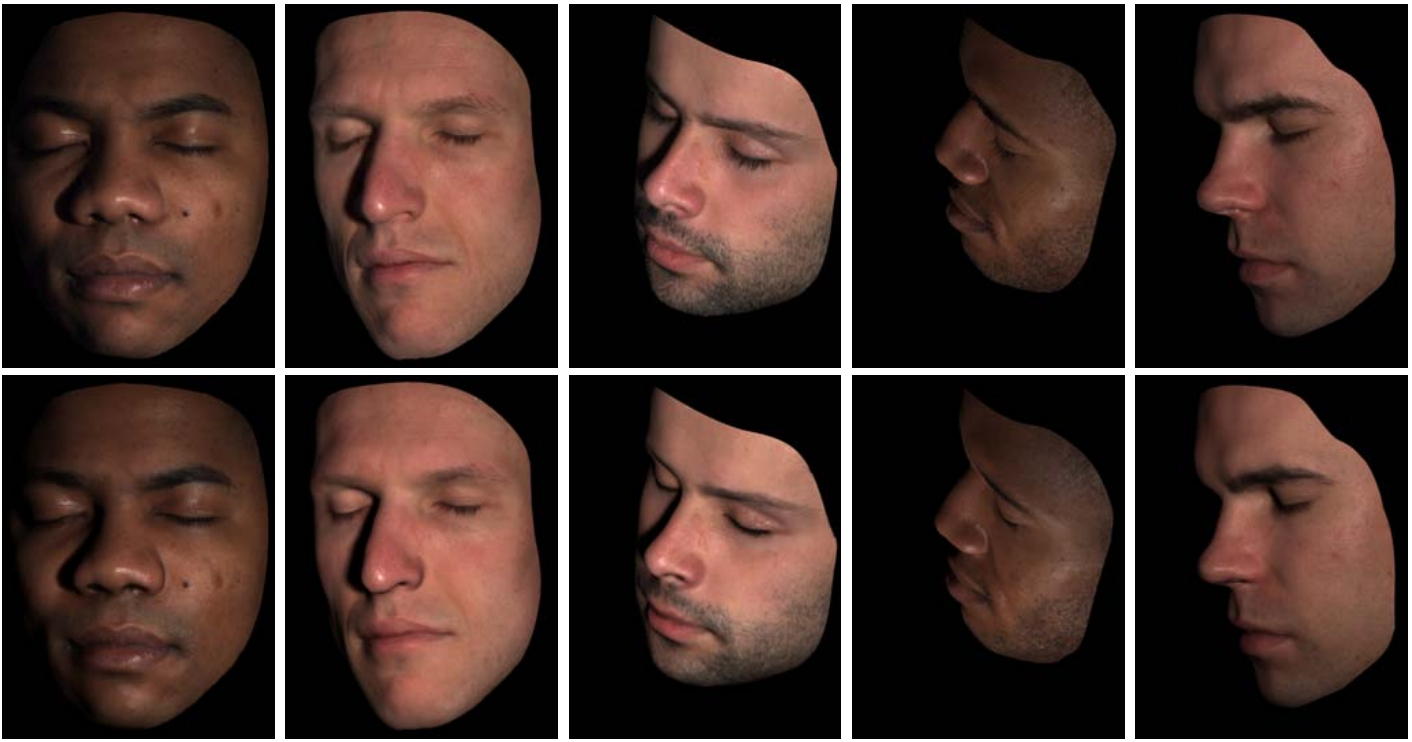
\includegraphics[scale=0.275,keepaspectratio]{./images/monte-carlo-ray-tracer.jpg}
\caption{A \enquote{Monte Carlo offline ray tracer} implemented in \citet{weyrich2006analysis}. Top row shows photograph, bottom shows rendered images}
\end{figure}

\renewcommand{\bibsection}{\section{Referenzen}} % requried for natbib to have "References" printed and as section, not chapter
% Use natbib compatbile splncsnat style.
% It does provide all features of splncs03, but is developed in a clean way.
% Source: http://phaseportrait.blogspot.de/2011/02/natbib-compatible-bibtex-style-bst-file.html
\bibliographystyle{splncsnat}
\begingroup
  \ifluatex
    %try to activate if bibliography looks ugly
    %\sloppy
  \else
    \microtypecontext{expansion=sloppy}
  \fi
  \small % ensure correct font size for the bibliography
  \bibliography{paper}
\endgroup

% Enforce empty line after bibliography
\ \\
%
All links were last followed on May 21, 2020.
\end{document}
